\documentclass[12pt]{article}

\usepackage[margin=1in]{geometry}
\usepackage{graphicx}
\usepackage{url}

\title{Rapid and accurate peptide identification from tandem mass spectra}

\author{Christopher Y. Park\footnote{These authors contributed equally 
to this work}\\
Department of Genome Sciences\\
University of Washington\\
Seattle, WA, USA
\and
Aaron A. Klammer$^*$\\
Department of Genome Sciences\\
University of Washington\\
Seattle, WA, USA
\and
Lukas K\"{a}ll\\
Department of Genome Sciences\\
University of Washington\\
Seattle, WA, USA
\and
Michael J. MacCoss\\
Department of Genome Sciences\\
University of Washington\\
Seattle, WA, USA
\and
William S. Noble\footnote{To whom correspondence should
  be addressed}\\
Department of Genome Sciences\\
Department of Computer Science and Engineering\\
University of Washington\\
Seattle, WA, USA
}

\begin{document}

\maketitle

\noindent Running title: {\sc Rapid, accurate peptide identification}

\noindent Keywords: Mass spectrometry, peptide identification, proteomics,
  bioinformatics

\clearpage

\begin{abstract}

\noindent
Mass spectrometry, the core technology in the field of proteomics,
promises to enable scientists to identify and quantify the entire
complement of proteins in a complex biological sample.  Currently, the
primary bottleneck in this type of experiment is computational.
Existing algorithms for interpreting mass spectra are slow and fail to
identify a large proportion of the given spectra.  We describe a
database search program called Crux that reimplements and extends the
widely used database search program {\sc Sequest}.  For speed, Crux
uses a peptide indexing scheme to rapidly retrieve candidate peptides
for a given spectrum.  For each peptide in the target database, Crux
generates shuffled decoy peptides on the fly, providing a good null
model and, hence, accurate false discovery rate estimates.  Crux also
implements two recently described post-processing methods: a $p$~value
calculation based upon fitting a Weibull distribution to the observed
scores, and a semi-supervised method that learns to discriminate
between target and decoy matches.  Both methods significantly improve
the overall rate of peptide identification.  Crux is implemented in C
and is distributed with source code freely to non-commercial users.
\end{abstract}

\clearpage

\section{Introduction}

Tandem mass spectrometry is the method of choice for many protein
identification studies.  However, this technology suffers from an
analysis bottleneck, with a need for more efficient and more accurate
methods of mapping from the observed fragmentation spectra to the
corresponding peptides.

The most widely used methods for peptide identification, such as {\sc
Sequest} \cite{eng:approach}, MASCOT \cite{perkins:probability},
X!Tandem \cite{craig:tandem}, Inspect \cite{tanner:inspect} and Lookup
Peaks \cite{bern:lookup}, exploit a database of known protein
sequences.  For each observed spectrum, these methods search the
database for the peptide whose theoretical spectrum best matches the
observed spectrum.  The resulting peptide-spectrum matches (PSMs) can
be ranked using a predefined score function, or by using machine
learning methods such as linear discriminant analysis
\cite{keller:empirical}, support vector machines \cite{anderson:new,
kall:semi-supervised} or decision trees \cite{elias:intensity}.

\begin{figure*}
\centering
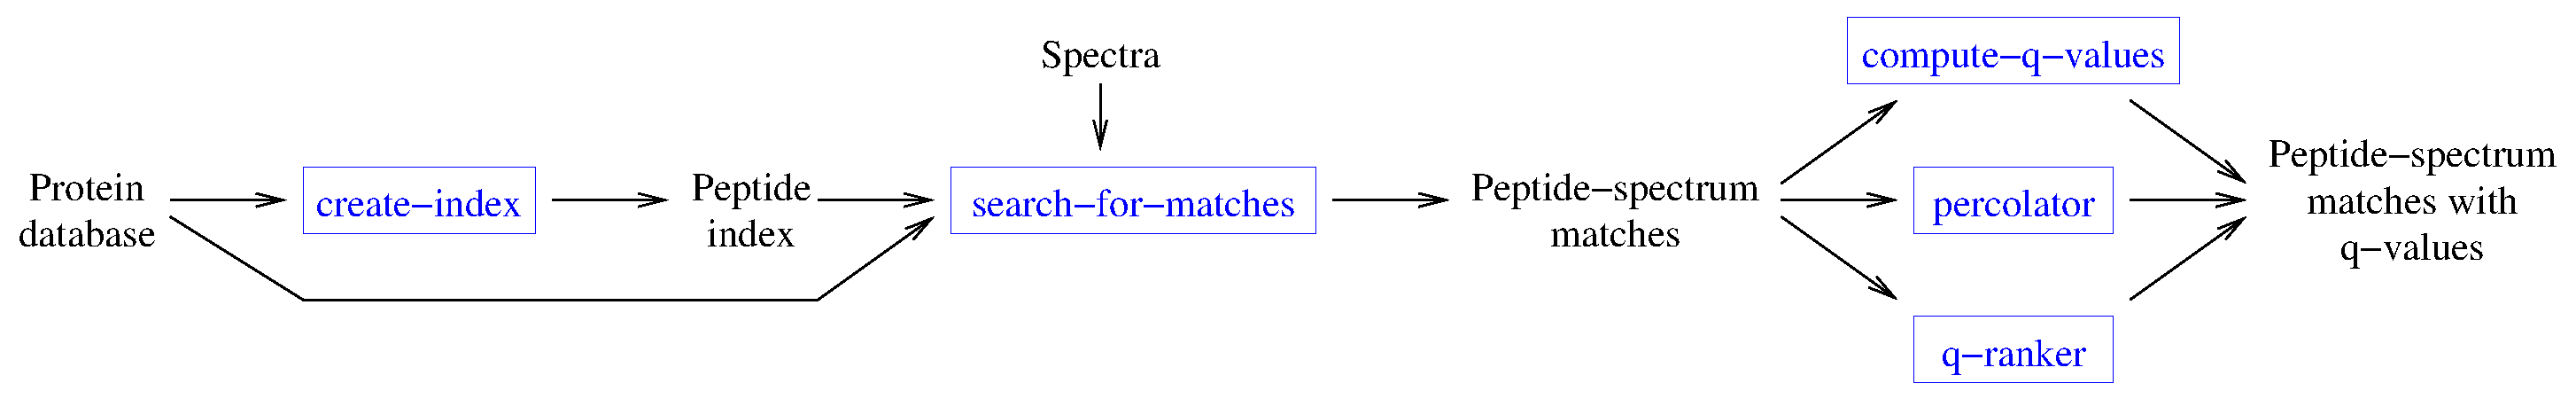
\includegraphics[width=6.5in]{schematic.eps}
\caption{{\bf The Crux algorithm.}  Crux takes as input a collection
  of fragmentation spectra and a target protein sequence database, and
  produces a list of peptide-spectrum matches, each with an associated
  $q$~value, a measure of false discovery rate. 
  \label{figure:crux}}
\end{figure*}

In this work, we describe a computational tool called Crux that solves
the peptide identification problem efficiently and accurately.
Figure~\ref{figure:crux} is a schematic diagram of Crux's work flow.
Crux's key features include the following:

\begin{itemize}
\item {\bf Efficient retrieval of candidate peptides.}  Given a
  spectrum with a specified precursor mass-to-charge ratio (m/z) and
  an assumed charge, Crux uses a precomputed peptide database to
  retrieve efficiently all peptides whose mass lies within a
  user-specified window around the target mass (called {\em candidate
  peptides}).  The database is sorted by peptide mass and is stored on
  disk, with mass indices stored in memory.  We show that, relative to
  {\sc Sequest}'s strategy of reading the protein sequence database
  from disk for each new spectrum, the indexed database decreases
  candidate peptide retrieval time from the human protein database by
  79.5\%--97.2\%, depending upon the width of the selected mass
  window.  Running under Windows, Crux's running time is comparable to
  that of Turbo{\sc Sequest}.

\item {\bf On-the-fly generation of decoy peptides.}  In evaluating
  the statistical significance of a PSM, mass spectrometrists
  frequently employ a {\em decoy database} comprised of protein
  sequences that have been reversed \cite{moore:qscore}, shuffled
  \cite{klammer:effects} or generated from a Markov chain derived from
  the given {\em target database} \cite{colinge:olav}.  The number of
  matches to the decoy database yields an estimate of the false
  discovery rate associated with a collection of target PSMs.  Crux
  uses this target-decoy strategy, generating decoys by shuffling the
  target peptides.  This approach ensures that each decoy peptide
  exhibits precisely the same amino acid composition and total mass as
  the corresponding target decoy.  To avoid the memory overhead
  associated with storing shuffled, non-overlapping decoy peptides in
  memory, Crux generates decoy peptides on the fly.

\item {\bf Two state-of-the-art PSM re-ranking algorithms} After
  scoring all peptides with respect to a given spectrum, the
  top-ranked PSM must be ranked with respect to other PSMs from the
  same data set.  Some score functions, such as {\sc Sequest}'s
  cross-correlation score ($XCorr$), have been used to carry out both
  relative ranking and absolute ranking; however, numerous studies
  have demonstrated that better absolute rankings can be achieved by
  using machine learning methods \cite{keller:empirical, anderson:new,
  elias:intensity, kall:semi-supervised}.  Crux incorporates two
  recently described methods for re-ranking PSMs.  The first method,
  called Percolator \cite{kall:semi-supervised}, trains a machine
  learning method to discriminate between target and decoy PSMs.  This
  dynamically trained model incorporates specific characteristics of
  the given data set.  The second method fits the observed $Xcorr$
  scores to a Weibull distribution and uses the resulting distribution
  to compute accurate $p$~values \cite{klammer:not}.

\item {\bf Accurate false discovery rate estimates.}  Crux uses
  well-established statistical methods to estimate false discovery
  rates based upon decoy PSMs \cite{benjamini:controlling}.  Crux
  reports, along with each PSM, a $q$~value, which is defined as the
  minimal false discovery rate threshold at which a given PSM is
  deemed correct \cite{storey:statistical}.  Depending upon the
  post-processing method, Crux estimates these $q$~values either using
  decoy PSMs or, for the Weibull curve fitting, directly from the
  estimated $p$~values.

\end{itemize}

Perhaps most significantly, from the perspective of the mass
spectrometry research community, Crux provides all of the above in a
stand-alone C program which is distributed, with source code, free for
non-commercial use (\url{http://noble.gs.washington.edu/proj/crux}).
Below, we demonstrate that Crux can accurately emulate {\sc Sequest},
and that Crux is both efficient and accurate, yielding a significant
improvement in running time and an increase in the number of correctly
identified spectra.

\section{Materials and Methods}

All Linux experiments were performed on a using a single CPU of a 2 x Intel
Xeon 2.33GHz 4-core processor machine with 4MB cache and 16GB of RAM
running RedHat Linux. All Windows experiments were performed using 
a Dell OptiPlex 745 Windows XP machine with an Intel Core 2 Duo E6400
processor (2.13 GHz, 2MB L2) and 2GB RAM with OpenSSH/Cygwin installed.

Using Crux, we precomputed a peptide database for two protein sequence
databases: the predicted open reading frames from yeast {\em
Saccharomyces cerevisiae} (released 2004-04-02, 3.6MB, 6298 proteins)
and human (released 2004-04-21, 16.8MB, 27209 proteins).  The indexes
contained tryptic peptides of length 6--50 amino acids and mass
200.0--7200.0 Da while allowing missed cleavage sites.  The indexing
procedures required, respectively, approximately two and four minutes
of real time and produced indices of 69 and 240 MB in size.

For validation, we use a publicly available tandem mass spectrometry
data set from \cite{klammer:improving}, available as the $60cm$ data
set at
\url{http://noble.gs.washington.edu/proj/retention/data/data.html}.
The data set consists of a collection of 18,149 spectra derived from a
analysis of soluble yeast whole-cell lysate on an LTQ ion trap mass
spectrometer as described previously \cite{klammer:improving}.

\section{Results}

\subsection{Efficient retrieval of candidate peptides}

When presented with a new query spectrum and its associated precursor
mass, Crux must first retrieve from the sequence database all of the
candidate peptides, i.e., peptides whose masses lie within a specified
range of the precursor mass.  A straightforward retrieval method is to
read the entire database from disk for each query, evaluating
candidate peptides as they are encountered.  This approach, which is
used by {\sc Sequest}, is space-efficient but can be slow for large
databases or large numbers of query spectra.

In addition to implementing the above approach, Crux offers an
alternative strategy that allows for more efficient candidate peptide
retrieval.  In this approach, the user must pre-process a given
protein database to produce a binary protein database and a binary
peptide index.  The pre-processing step sorts all of the peptides in
the database by mass and stores pointers to their locations in the
protein database (sequence index, start position, and peptide length).
Crux can then quickly retrieve a set of candidate peptides via a
simple range query on the peptide index.  Upon execution, Crux
accesses the binary protein database and the peptide index as
memory-mapped files.  This approach offloads to the operating system
the decision about how much of the database to store in memory,
ensuring that small databases are read fully into memory but large
databases are paged into and out of memory only as needed.

\begin{figure}
\centering
\begin{tabular}{l}
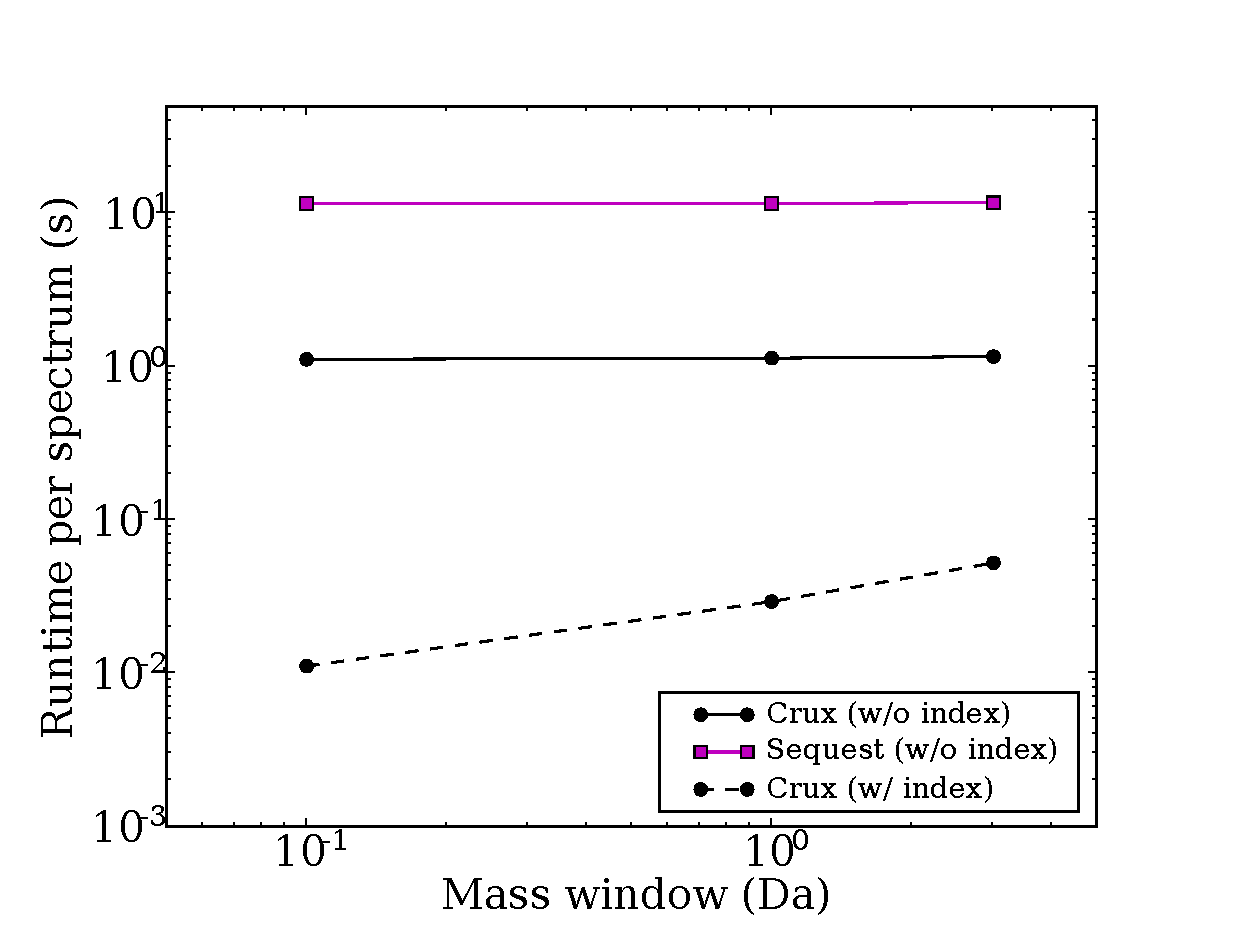
\includegraphics[width=2.5in]{../../results/paper-figure/index/indexing-human.eps} \\
{\sf (A)} Linux \\
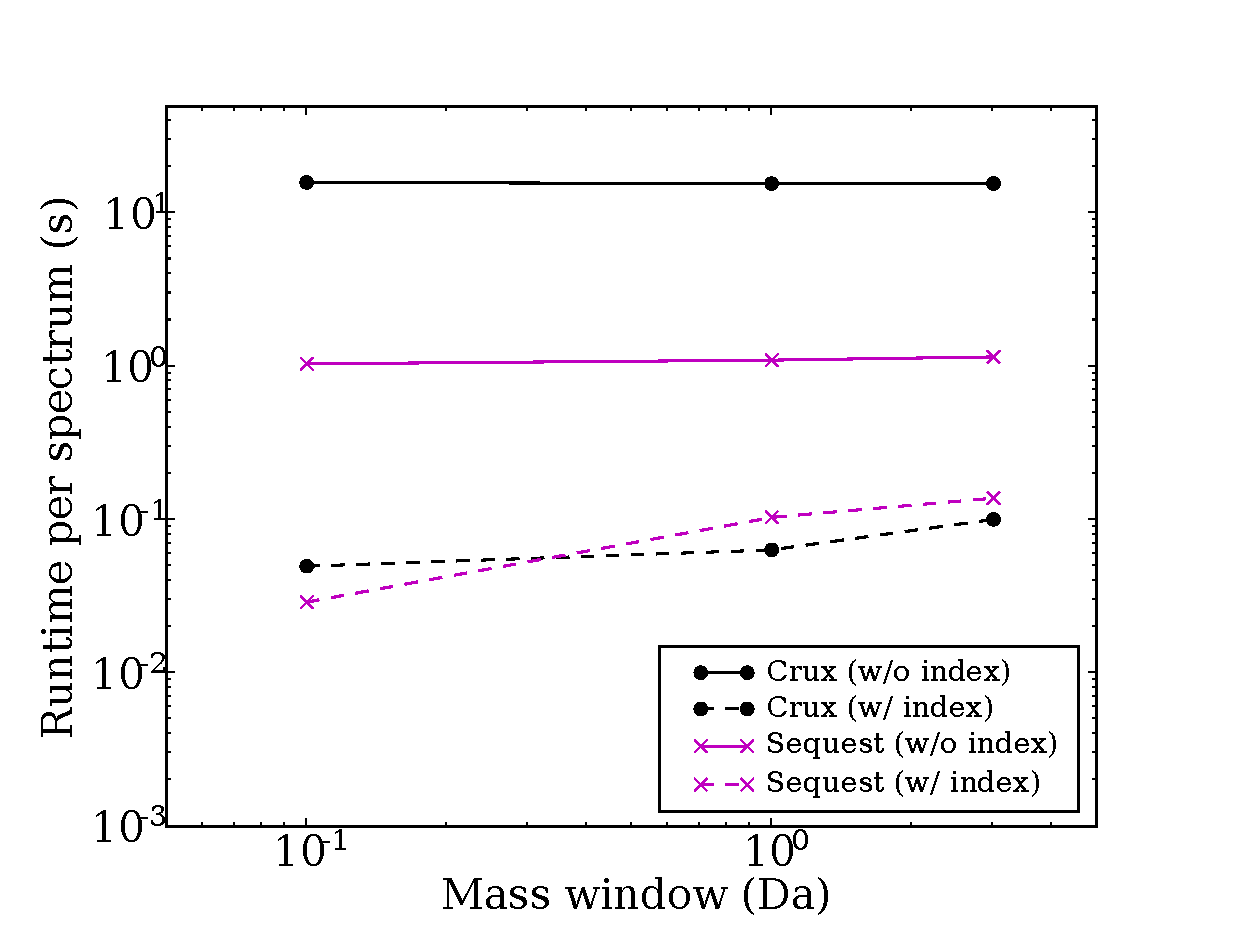
\includegraphics[width=2.5in]{../../results/paper-figure/turbo-no-missed-human/indexing-yeast-windows.eps} \\
{\sf (B)} Windows \\
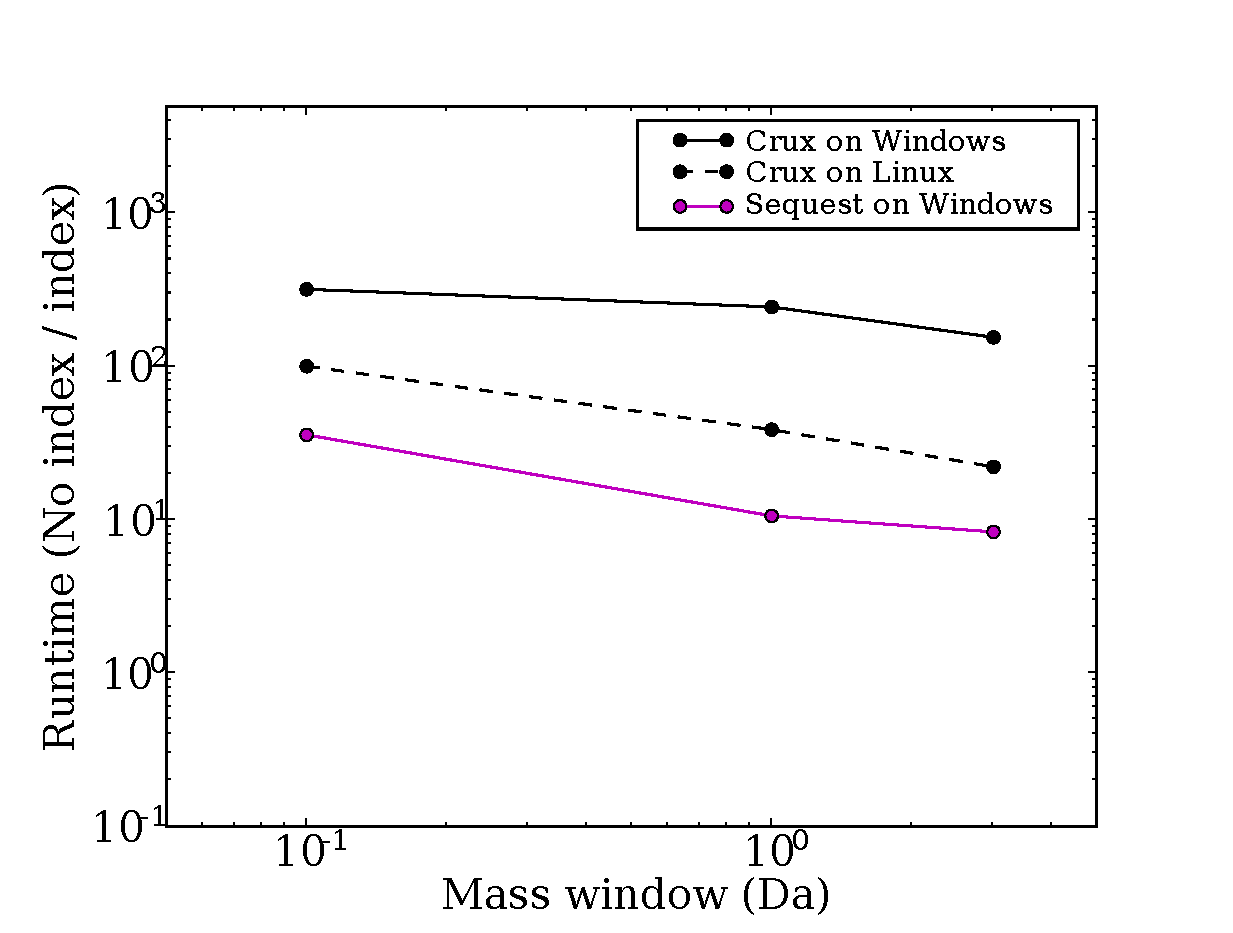
\includegraphics[width=2.5in]{../../results/paper-figure/comparison/ratio.eps} \\
{\sf (C)} \\
\end{tabular}
\caption{{\bf Rapid retrieval of candidate peptides.}  Panels (A) and
  (B) plot the average running time required to search 100 tandem mass
  spectra against the human protein databases on computers running the
  Linux ({\sf A}) or Windows ({\sf B}) operating systems, using {\sc
  Sequest} and Crux with and without indices.  Running time is plotted
  as a function of the mass tolerance used to define candidate
  peptides. The Linux plot includes only three series because we do
  not have a Linux implementation of Turbo{\sc Sequest}.  {\sf (C)} The
  figure plots ratio of running times for non-indexed versus indexed
  searches for Crux on Windows and Linux and for {\sc Sequest} on Windows.
  \label{figure:indexing}}
\end{figure}

%---------------------------------
% Indexing numbers for human
% 
% Crux w/index
%
% 0.10000000      32.35000000
% 1.00000000      96.41000000
% 3.00000000      241.14000000
% 
% Crux w/o index
% 
% 0.10000000      16245.42000000
% 1.00000000      16230.78000000
% 3.00000000      16225.12000000
% 
% Sequest
% 
% 0.10000000      1161.42000000
% 1.00000000      1164.75000000
% 3.00000000      1174.11000000
%---------------------------------

To demonstrate the efficiency of Crux's candidate peptide retrieval
strategy, we searched with a collection of 100 spectra against
predicted human protein sequences from the human genome, generating
candidate peptides from a series of increasingly wider mass windows.
Figure~\ref{figure:indexing}A plots the average search time per spectrum 
running under
Linux as a function of mass window width. Analogous plots with similar
trends for a search against the yeast {\em Saccharomyces cerevisiae}
are shown in the online supplement.  In general, Crux runs more
quickly than {\sc Sequest}, and the improvement is larger when Crux
uses a peptide index.  The difference in running time is most
pronounced when the mass tolerance window is small, because Crux does
not need to scan the entire database to retrieve a small collection of
candidate peptides.  For example, with a mass tolerance window of 0.1,
on Linux {\sc Sequest} 
requires an average of 11.6~s clock time per spectrum, whereas Crux requires
an average of 10~ms. 
This represents a 99.9\% reduction in running time. However,
even when we use a mass tolerance of 3, Crux yields a 99.5\% speed
improvement (52~ms versus 11.7~s).

Crux is not the first attempt to improve the speed of candidate
peptide retrieval.  Thermo Scientific (Waltham, MA) markets a version
of {\sc Sequest} called Turbo{\sc Sequest} as part of the Bioworks 3.1
software, which implements a peptide index using a proprietary scheme.
In Figure~\ref{figure:indexing}B, we compare Crux to Turbo{\sc Sequest}
under Windows XP.  Execution of Crux on Windows was performed from
within the Unix emulator Cygwin, which induces a slight overhead.
This may explain, in part, the reversal between the non-indexed
versions of Crux and {\sc Sequest} between panels A and B: under
Windows in this mode, {\sc Sequest} runs significantly more quickly
than Crux.  Nonetheless, with indexing Crux's speed is comparable to
that of Turbo{\sc Sequest}.  In Figure~\ref{figure:indexing}C we directly
assess the speedup due to indexing, plotting the ratio of the running
time with and without indexing for Crux under Linux and Windows and
for {\sc Sequest} under Windows.  For all three mass window sizes,
Crux achieves a much larger speedup than {\sc Sequest}.

A surprising property of Figure~\ref{figure:indexing}A--B is the
flatness of the two series corresponding to {\sc Sequest} and Crux
without an index.  This flatness indicates that the running time for
retrieving candidate peptides is dominated by the fixed cost
associated with scanning the file from disk.  Relative to this fixed
cost, the time required to calculate the preliminary score $Sp$ is
negligible.

\subsection{Accurate reimplementations of $Sp$ and $Xcorr$}

{\sc Sequest} is the first and one of the most widely used database
search methods for peptide identification from tandem mass spectra.
Crux therefore begins with a reimplementation of the core of {\sc
Sequest}.  After retrieving all of the candidate peptides for a given
spectrum, the candidates are ranked according to the preliminary {\sc
Sequest} score $Sp$.  Subsequently, the 500 top-scoring peptides are
re-ranked according to the cross-correlation score $XCorr$.

For $Sp$ scoring, Crux applies a series of pre-processing steps to the
observed spectrum.  We summarize the main operations here.  First,
Crux takes the square root of each peak's intensity and rounds each
peak's m/z to the nearest integer.  Second, Crux normalizes the peak
intensities to sum to 100.  Third, Crux extracts the top 200 highest
intensity peaks.  Crux compares the resulting observed spectrum $v$
with the b and y fragment ions $u$ from the candidate peptide to
compute $Sp$ as follows:
\[
S_p(u, v) = \frac{
\left(\sum_{i=1}^N v_i \delta(u_i) \right)
\left(\sum_{i=1}^N \delta(u_i v_i)\right)
\left(1 + 0.075 R(u, v) \right)
}{\sum_{i=1}^N \delta(u_i)}
\]
where $N$ is the maximal m/z value, $R(u, v)$ is the maximum number of
consecutive b- or y-ions from the theoretical spectrum that appear in
the observed spectrum, and $\delta(x) = 0$ if $x=0$ and $\delta(x) =
1$ otherwise.

$Xcorr$ scoring also requires some pre-processing of the observed
spectrum.  As before, Crux first takes the square root of each peak's
intensity and rounds each peak's m/z to the nearest integer.  Second,
Crux divides the spectrum into 10 regions and normalizes the spectrum
intensity in each region to maximum of 50.0. To create the theoretical
spectrum from the candidate peptide, Crux constructs a spectrum with
peak intensity 50.0 for b and y ions, 25.0 for the $\pm 1$ m/z flanking
peaks of each b and y ion, and 10.0 for ions resulting from a neutral
loss of ammonia from b or y ions or neutral loss of water from b ions.
Crux then computes $Xcorr$ as follows:
\[
X_c(u, v) = \frac{0.015\sum_{i=1}^N u_i v_i}
{\sum_{\tau=-75}^{75} \sum_{i=1}^N u_i v_{i-\tau}}
\]

\begin{figure*}
  \centering
  \begin{tabular}{ll}
    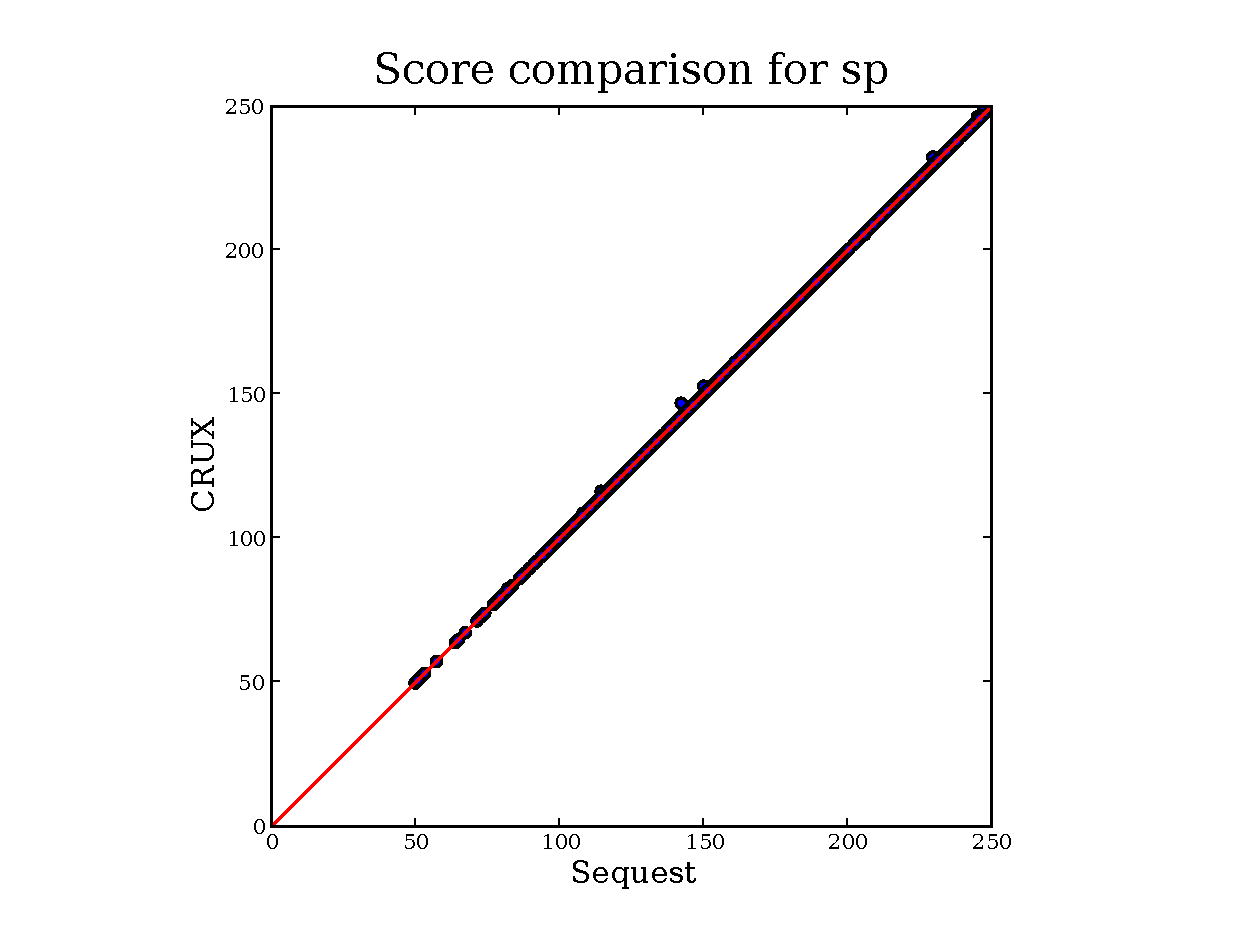
\includegraphics[width=3in]{./Images/random-sp.eps} &
    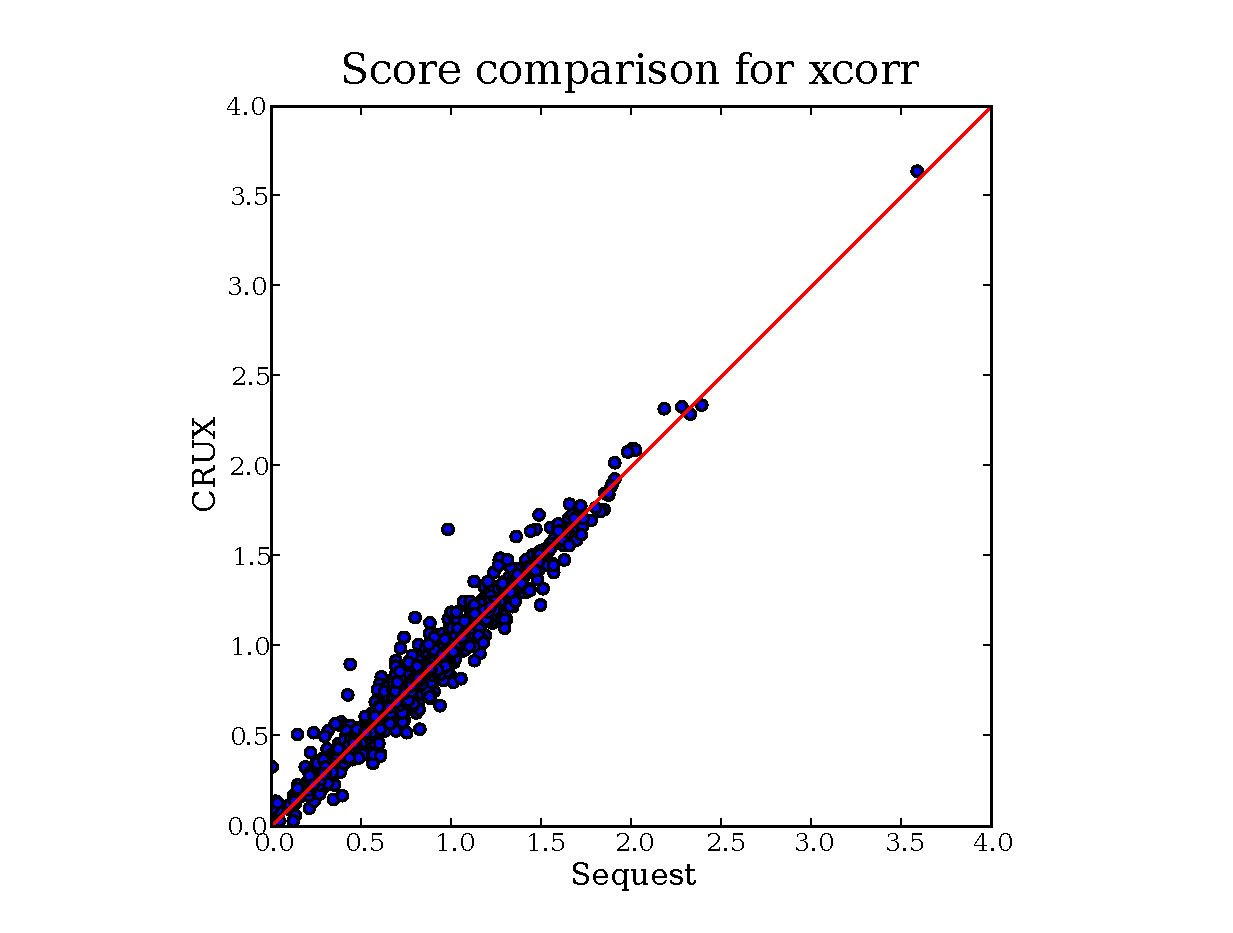
\includegraphics[width=3in]{./Images/random-xcorr.eps} \\
    {\sf A} & {\sf B}\\
  \end{tabular}
  \caption{{\bf Re-implementation of $Sp$ and $Xcorr$ scoring functions.}
  The figure plots, for a collection of peptide-spectrum matches, the
  $Sp$ ({\sf A}) and $XCorr$ ({\sf B}) scores as computed by Crux as a function of the
  same scores as computed by {\sc Sequest}.
  \label{figure:sp-xcorr}}
\end{figure*}
Figure~\ref{figure:sp-xcorr} shows that the Crux-calculated versions
of $Sp$ and $Xcorr$ closely match the {\sc Sequest}-calculated
versions of these scores. We also analyzed 
MALDI-TOF/TOF and QTOF spectra from \citep{klimek:standard} against the
same database, in order to more fully sample the space of
possible PSMs, and again our Crux-calculated scores are similar to the
{\sc Sequest} versions (see the online supplement). The vast majority
of the PSMs receive identical scores using either method.
Furthermore, as shown in Figure~\ref{figure:pq-plot} (described in
Section~\ref{section:experimental}), the Crux and {\sc Sequest}
algorithms perform very similarly in practice.

\subsection{Null peptide generation}
\label{section:on-the-fly}

When identifying peptides from tandem mass spectra, a commonly used
null model is to search the given set of spectra against a {\em decoy
database}.  A decoy database is a database of amino acid sequences
that is derived from the original protein database (called the {\em
target database}) by reversing the target sequences
\cite{moore:qscore}, shuffling the target sequences
\cite{klammer:effects}, or generating the decoy sequences at random
using a Markov model with parameters derived from the target sequences
\cite{colinge:olav}.  Ideally, the decoy database should contain
peptide-like amino acid sequences that are not in the target database.

Crux uses a decoy strategy; however, rather than generating a fixed
decoy database, Crux generates decoys on the fly.  For each comparison
between a spectrum and a target peptide, Crux generates a
corresponding decoy peptide by shuffling the non-terminal amino acids
of the target peptide.  Consequently, Crux reports for every target
PSM one or more corresponding decoy PSMs.  On-the-fly decoy generation
introduces a small computational overhead but saves space, because the
decoy database does not need to be stored.

X!Tandem \cite{craig:tandem} will automatically generate a reversed
decoy database from the given database, but by definition a reversed
decoy database can only be generated once for a given database.
Crux, in contrast, generates a new shuffled decoy peptide for every
peptide-spectrum comparison.  Thus, if a particular peptide is
selected as a candidate for 100 different spectra, then it will be
shuffled 100 different times.  This approach eliminates the
possibility that a single decoy peptide will match well against many
spectra.

An additional advantage of generating decoys on the fly is that the
resulting decoys share exactly the same total mass and amino acid
composition as the target.  When using a static decoy database,
ensuring that the target and decoy peptide mass and amino acid
composition stays the same is very difficult.  For example, shuffled
and Markov chain-generated decoy databases will not retain these
properties. A reversed database will retain these properties, but only
when trypticity is not enforced.  On-the-fly decoy generation has the
further advantage that, unlike reversed decoys, multiple decoys can be
generated for a single target.  These additional decoys can be useful
if the user wants more accurate confidence estimates.

\subsection{Methods for post-processing peptide-spectrum matches}
\label{section:post-process}

Identifying peptides from tandem mass spectra via database search is,
fundamentally, a ranking procedure, in which good PSMs are ranked
above poor PSMs.  This ranking task can be usefully separated into two
phases: a {\em relative ranking} task, in which all of the candidate
peptides are ranked relative to a single spectrum to identify a single
best PSM for that spectrum, and an {\em absolute ranking} task, in
which the top-ranked PSMs for multiple spectra are ranked relative to
one another.  Absolute ranking is, by definition, more difficult than
relative ranking.  Furthermore, empirical evidence suggests that,
although $Xcorr$ does a good job at relative ranking, it performs more
poorly when attempting to rank PSMs absolutely \cite{keller:empirical,
anderson:new}. Crux therefore implements two recently described
methods for post-processing PSMs to improve their absolute ranking.

The first post-processor is a semi-supervised machine learning method
called Percolator that dynamically learns an absolute PSM ranking
function \cite{kall:semi-supervised}.  Percolator uses a subset of the
high-scoring target PSMs as positive examples and all of the decoy
PSMs as negative examples to train a discriminative classification
algorithm called a support vector machine (SVM) \cite{boser:training,
noble:what}.  Each PSM is characterized using a collection of features
that capture characteristics of the spectrum, the peptide, and the
quality of the match between the spectrum and the peptide.  Details of
the Percolator algorithm are given in \cite{kall:semi-supervised}.

The second post-processing method fits the observed distribution of
candidate PSM $Xcorr$ scores to a Weibull distribution.  To do this
fitting in an unbiased way, Crux computes 500 additional $Xcorr$ scores
at random from the candidate set, in addition to scoring the top 500
candidates selected by $Sp$.  The resulting Weibull distribution is
then used to compute a $p$~value for the observed maximum score, and
the score is further corrected to account for the total number of
candidates that were considered.  Details of this $p$~value estimation
procedure are given in \cite{klammer:not}.

Crux produces as output a ranked list of target PSMs, one per spectrum
in the given data set.  Along with each PSM, Crux reports a $q$~value,
which is defined as the minimal false discovery rate at which this PSM
is called positive \cite{storey:statistical, kall:assigning}.  False
discovery rates are estimated using the method of
\cite{benjamini:controlling}.  When running without post-processing,
the null distribution is estimated using the decoy PSMs.  When
Percolator is used, half of the decoy PSMs are used to train the
classifier, and half are used to estimate the final $q$~values.  For
the empirical $p$~value calculation, decoy PSMs are not necessary,
because the FDR can be estimated directly from the computed
$p$~values.  Eliminating the decoys leads to an approximately 50\%
decrease in running time for this search mode versus the standard
target-decoy search approach.

\subsection{Experimental comparison of methods}
\label{section:experimental}

\begin{figure}
\centering
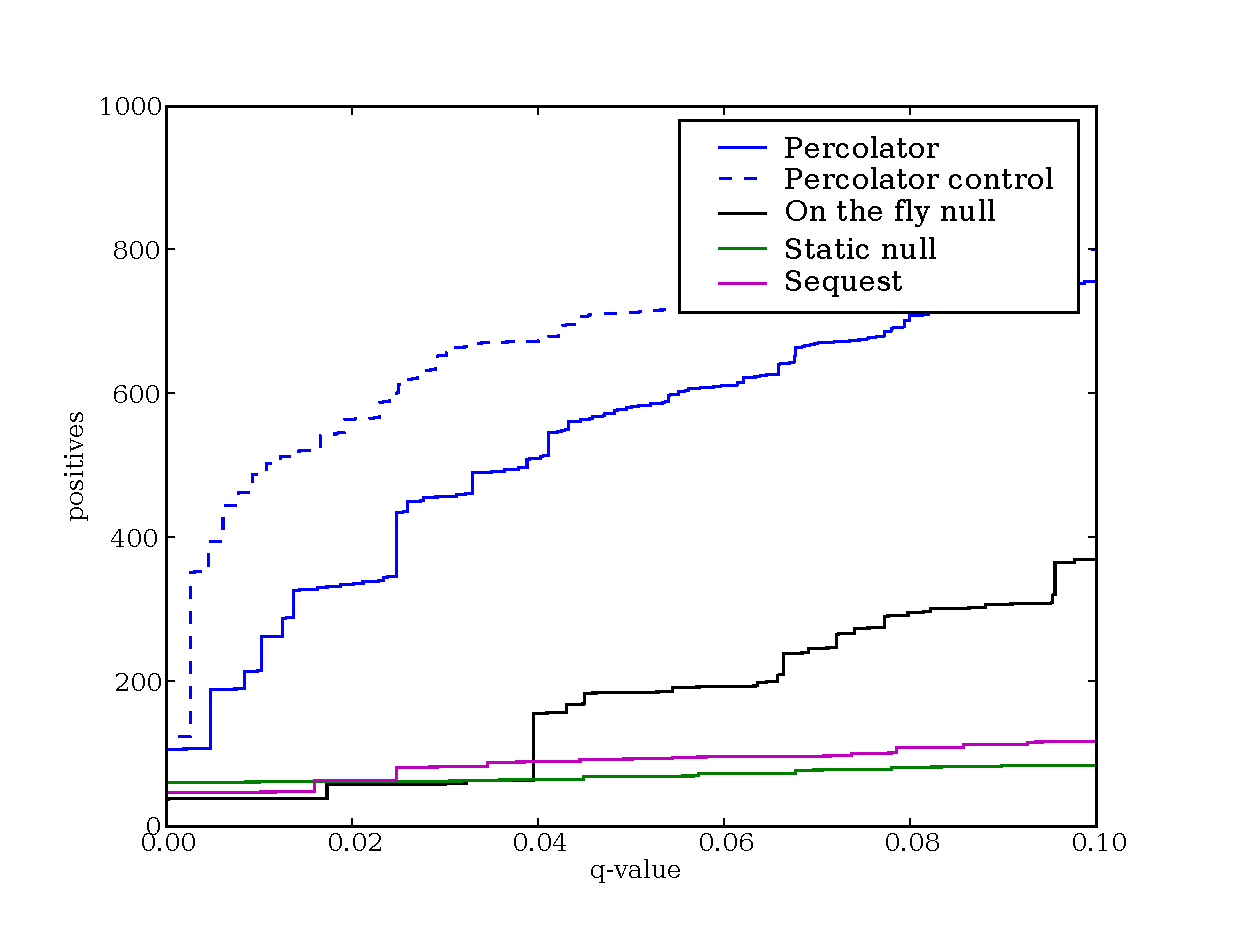
\includegraphics[width=5in]{./Images/q-value.eps}
\caption{{\bf Improved peptide identification.}  The figure plots, for
  a variety of database search algorithms, the number of PSMs as a
  function of the estimated $q$~value.  The five series correspond to
  {\sc Sequest}, Crux's implementation of {\sc Sequest} using a static
  shuffled decoy database, Crux using decoys generated on-the-fly,
  Crux with the $p$~value calculation enabled, and Crux with the
  Percolator post-processor enabled.
  \label{figure:pq-plot}}
\end{figure}

To compare the performance of {\sc Sequest} and the various algorithms
implemented in Crux, we used a collection of 18,149 spectra derived
from a yeast whole-cell lysate (see Methods).  Each peptide
identification method searches against the yeast proteome and produces
a list of 35,676 PSMs ranked by $q$~value, computed as described in
Section~\ref{section:post-process} (the number of spectra differs from
the number of PSMs because some spectra are searched multiple times,
once for each possible charge state).  For {\sc Sequest} and for Crux
with a static decoy database, we use a decoy database of shuffled
proteins.  Figure~\ref{figure:pq-plot} plots, for each method, the
number of accepted PSMs as a function of $q$~value threshold.

Three of the series in Figure~\ref{figure:pq-plot} lie very close to
one another.  The similarity between the results given by {\sc
Sequest} and the Crux reimplementation of {\sc Sequest} provides
evidence that Crux accurately reimplements the {\sc Sequest}
algorithm.  The series corresponding to on-the-fly decoy generation is
also essentially identical to the two series generated using static
decoys.  Although the on-the-fly decoy generation does not lead to
better results, we believe that it is a better null model, for the
reasons given in Section~\ref{section:on-the-fly}.  We therefore use
this null model by default in Crux.

Finally, consistent with previously reported results
\cite{klammer:not, kall:semi-supervised}, the $p$~value calculation
yields a large improvement over simple ranking by $Xcorr$, and using
Percolator yields an even more dramatic improvement.  At a $q$~value
threshold of 0.01, $Xcorr$ ranking yields 1,609 PSMs, ranking by
$Xcorr$ $p$~values yields 4,904 PSMs, and ranking by Percolator score
yields 6,294 PSMs.  It is not surprising that Percolator performs
better than the $p$~value calculation, because Percolator exploits a
wide variety of PSM features, whereas the $p$~value is based only on
the observed $Xcorr$ distribution and the number of candidate
peptides.  On the other hand, the $p$~value calculation is roughly
twice as fast as all of the other methods reported here, because the
$q$~values are calculated analytically, rather than by searching a
decoy database.

\section{Discussion}

One practical challenge impeding research on mass spectrometry peptide
identification algorithms is that source code for two of the most
widely used algorithms---{\sc Sequest} and MASCOT---are not publicly
available.  For non-commercial users, Crux remedies this situation,
while also making available a fast candidate peptide retrieval
algorithm and several state-of-the-art post-processing algorithms.
Although Crux is implemented in C, the code design is object oriented.
The core of the Crux search engine is currently $Sp$
and $Xcorr$, but the code modules for candidate retrieval or
post-processing could be easily modified to work with alternative
searching algorithms.

Recently, several groups have described an alternative
approach to candidate peptide retrieval using metric space embeddings
\cite{ramakrishnan:fast, dutta:speeding}.  These approaches promise
even larger speedups at the expense of failing to retrieve a small
fraction of the candidate peptides.

The comparison of post-processing methods in
Figure~\ref{figure:pq-plot} shows that Percolator significantly
improves upon the $p$~value-based ranking.  However, computing
$p$~values has the advantage of cutting the overall search time in
half by eliminating the need for a decoy database.  One could imagine
coupling these two post-processing algorithms by providing $p$~values
as inputs to Percolator; however, doing so would require decoy PSMs to
train Percolator.  Hence, we believe that decoy database searching
will continue to be a valuable component of database searching, even
in the presence of analytically calculated significance measures.

Crux is under development, and several significant enhancements are
planned for the near future.  Some are straightforward, including
allowing alternative file formats for input and output (currently,
Crux uses the MS2 and SQT file formats \cite{mcdonald:ms1}), improved
support for searches that allow multiple masses per amino acid, and
parallelization of the code. Our indexing strategy was specifically
designed with the latter in mind: the parallelization will divide the
database among processors, sending each observed spectrum to the
processor that stores the appropriate mass range.  We also plan to
extend the peptide index to allow for storage of additional pieces of
precomputed information, such as predicted peak intensities,
predicted peptide retention time, or predicted proteotypic peptides
\cite{mallick:computational}.  Finally, we have plans for algorithmic
improvements, including increasing the variety of features used by
Percolator, improving the accuracy of our $q$~value estimates using
existing methods \cite{storey:direct}, and implementing algorithms for
protein-level identification.

\section*{Acknowledgments}
We thank Jimmy Eng for useful discussions.

\section*{Funding}
NIH awards P41~RR11823 and R01~EB007057.

\bibliographystyle{plos}
\bibliography{refs} 

\end{document}
